\documentclass[11pt]{exam}
\usepackage[spanish]{babel}
\usepackage[utf8]{inputenx}
\usepackage{fontenc}
\usepackage{textcomp}
\usepackage{lmodern,pifont}
\usepackage{graphicx}
\graphicspath{ {./img_1479/} }
\usepackage{setspace}
\usepackage[dvipsnames]{color}
\usepackage{colortbl}
\usepackage{caption}
\usepackage{amsmath}

\newcommand\titexam[1]{\centering%
\fbox{\parbox{\textwidth}{\huge \sffamily \textbf{#1}}}\normalsize \vspace{1em}}

\renewcommand{\solutiontitle}{\noindent\textbf{Solución:}\par\noindent}

\pagestyle{empty}
\begin{document}
{\fontfamily{lmss}\selectfont
\textbf{INSTRUCCIONES:}
\begin{itemize}
    \item Se dispone de una hora para responder las 20 preguntas.
    \item Cada pregunta tiene un valor de 0.5 punto.
    \item Para considerar la respuesta como correcta, la opción escogida ha de
      estar correctamente señalada. Las preguntas erróneamente marcadas se
      considerarán como incorrectas. 
    \item Cada respuesta incorrecta resta 0.17 puntos. Las respuestas en blanco no restan. 
\end{itemize}
\vspace{1cm}

\titexam{MF1479\_2 Propagación de plantas en vivero}
\begin{questions}
  % 1
\question El nombre científico de una especie se forma de dos partes. ¿Puedes
indicar a que categoría taxonómica corresponde la primera parte?
\begin{checkboxes}
  \choice A. Al Reino
  \choice B. A la Familia
  \CorrectChoice C. Al Género
  \choice D. Ninguna es correcta
\end{checkboxes}
% 2
\question ¿Qué tipo de raíz aparece en la imagen?
  \begin{figure}[h!]
    \centering
    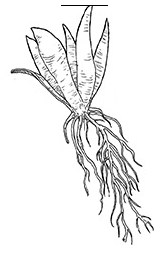
\includegraphics[width=0.2\textwidth]{fasciculada.PNG}
  \end{figure}
  \begin{checkboxes}
    \choice A. Napiforme
    \choice B. Pivotante
    \choice C. Ramificada
    \CorrectChoice D. Fasciculada
  \end{checkboxes}
  \newpage
  % 3
  \question ¿Como se llama la parte del tallo a partir de la cual se pueden
  desarrollar flores o tallos?
  \begin{checkboxes}
    \CorrectChoice A. Yemas
    \choice B. Nudos
    \choice C. Lenticelas
    \choice D. Ninguna respuesta es correcta
  \end{checkboxes}
  % 4
  \question ¿Como se llama la parte de la flor donde se forma y almacena el polen?
  \begin{checkboxes}
    \choice A. Cáliz
    \CorrectChoice B. Estambre
    \choice C. Tubo polínico
    \choice D. Gineceo
  \end{checkboxes}
  % 5
  \question ¿Qué ecosistemas son extremadamente sensibles a la contaminación por
  plantas invasoras y con las que hay que hay que extremar precauciones?
  \begin{checkboxes}
    \choice A. Ecosistemas de montaña
    \CorrectChoice B. Ecosistemas de agua dulce (ríos y sus
    riveras, lagos, humedales, etc)
    \choice C. Ecosistemas dunares
    \choice D. Ecosistema forestal
  \end{checkboxes}
  % 6
  \question Los nutrientes de un suelo se clasifican en macroelementos y microelementos. ¿A
  qué se debe el nombre de estos últimos?
  \begin{checkboxes}
    \choice A. A qué la mayoría de elementos son de pequeño tamaño
    \choice B. A qué tienen poca importancia para las plantas
    \choice C. A qué se encuentran en el suelo en poca proporción
    \CorrectChoice D. A qué se encuentran en las plantas en menor proporción 
  \end{checkboxes}
  % 7
  \question ¿La porosidad de un suelo es?
  \begin{checkboxes}
    \choice A. Una propiedad física de los suelos
    \choice B. Una cualidad que determina si el suelo drena en exceso
    \choice C. La relación del volumen de espacios vacíos de un suelo con
    respecto a su volumen total
    \CorrectChoice D. Las respuestas A y C son correctas
  \end{checkboxes}
  % 8
  \question Como afecta el pH del suelo a los elementos químicos presentes en el suelo?
  \begin{checkboxes}
    \choice A. Con pH más ácidos la mayoría de los nutrientes serán absorbidos más
    fácilmente
    \choice B. Afecta a la disponibilidad de nutrientes para las plantas.
    \choice C. Dependiendo del pH del suelo algunos nutrientes serán más fácilmente
    absorbidos por las plantas que otros
    \CorrectChoice D. Las respuestas B y C son correctas
  \end{checkboxes}
  \newpage
  % 9
  \question ¿Qué propiedad física del suelo depende del tamaño de las partículas que la
  componen?
  \begin{checkboxes}
    \CorrectChoice A. Textura
    \choice B. Porosidad
    \choice C. Estructura
    \choice D. Ninguna respuesta es correcta
  \end{checkboxes}
  % 10
  \question ¿Los tipos de riesgos que un operario corre por  realizar tareas de abonado del
  terreno pueden ser?
  \begin{checkboxes}
    \choice A. Sobreesfuerzos por manipular cargas o posturas inadecuadas
    \choice B. Contacto con agentes químicos o ingestión accidental de tóxicos
    \choice C. Lesiones en la piel por salpicaduras de residuos o agentes químicos
    \CorrectChoice D. Todas las respuestas son correctas
  \end{checkboxes}
  % 11
  \question ¿Qué tipo de ventajas supone la reproducción sexual frente a la
  vegetativa?
  \begin{checkboxes}
    \CorrectChoice A. Aumentar la variación genética de la especie ya que la
    descendencia es producto de los genes de ambos progenitores
    \choice B. Obtener plantas iguales
    \choice C. Que los gametos masculino y femenino se encuentren ya supone 
    un menor gasto energético en la reproducción lo que da como resultado una
    mayor rapidez del proceso
    \choice D. Todas las respuestas son correctas 
  \end{checkboxes}
  % 12
  \question Las semillas, según el contenido de humedad que han de retener para
  sobrevivir se clasifican en?
  \begin{checkboxes}
    \CorrectChoice A. Ortodoxas y recalcitrantes
    \choice B. Dehiscentes e indehiscentes
    \choice C. Simples y recalcitrantes
    \choice D. Las respuestas A y C son correctas
  \end{checkboxes}
  % 13
  \question ¿Qué es un tratamiento pregerminativo de semillas?
  \begin{checkboxes}
    \choice A. Una técnica que mejora la calidad de las semillas
    \CorrectChoice B. Un conjunto de técnicas que han de facilitar el germinado de las
    semillas
    \choice C. Un conjunto de técnicas que aumentan el vigor de las semillas
    \choice D. Todas las respuestas son correctas
  \end{checkboxes}
  % 14
  \question ¿Como se llama una característica propia de las semillas que las impide germinar
  incluso si las condiciones ambientales son favorables?
  \begin{checkboxes}
    \choice A. Vernalización
    \CorrectChoice B. Latencia
    \choice C. Damping-off
    \choice D. Anemocoria
  \end{checkboxes}
  \newpage
  % 15
  \question Además de poder controlar la presencia de hierbas no deseadas de forma manual o
  mecánica, ¿de qué otra manera podemos evitar la presencia de hierbas no deseadas sin
  emplear herbicidas?
  \begin{checkboxes}
    \choice A. Arranque
    \choice B. Siega
    \CorrectChoice C. Mulching o acolchados
    \choice D. Fumigando
  \end{checkboxes}
  % 16
  \question ¿Cuantas yemas debe contener como mínimo un esqueje o estaquilla para un correcto
  desarrollo y enraizado?
  \begin{checkboxes}
    \choice A. No importa el número de yemas, solo la calidad de la planta madre
    \choice B. Una
    \CorrectChoice C. Dos
    \choice D. Con una yema será suficiente siempre y cuando dejemos las hojas completas
  \end{checkboxes}
  % 17
  \question ¿Qué es un patrón?
  \begin{checkboxes}
  \choice A. Persona encargada de los trabajos en el campo
  \CorrectChoice  B. Planta que recibe un injerto y aporta el sistema radicular
  \choice C. Trozo de rama que se introduce en un pie o planta para reproducirla
  \choice D. Parte de una rama en la que hacemos una incisión para quitar un
  anillo y que cubrimos con sustrato ayudándonos de una bolsa.
  \end{checkboxes}
  % 18
  \question ¿Qué tipo de material se suele emplear para realizar las uniones de los
  injertos?
  \begin{checkboxes}
    \choice A. Alambre de acero
    \choice B. Teflón
    \CorrectChoice C. Rafia, goma elástica, cinta aislante, film transparente
    \choice D. Todas las respuestas son correctas 
  \end{checkboxes}
  % 19
  \question Las plantas tienen capacidad de reproducirse de manera asexual mediante
  ciertas estructuras tales como?
  \begin{checkboxes}
    \CorrectChoice A. Bulbos y tubérculos
    \choice B. Estacas y esquejes
    \choice C. Acodo y rizoma
    \choice D. Todas las respuestas son correctas 
  \end{checkboxes}
  % 20
  \question ¿Por qué es importante que los cuchillos para realizar injertos estén bien
  afilados?
  \begin{checkboxes}
    \CorrectChoice A. Para que los cortes ha realizar tanto en la púa como el patrón sean
    cortes limpios
    \choice B. Para poder cortar las ramas que sirvan para injertar
    \choice C. Para realizar cortes limpios en el material para unir los injertos
    \choice D. Para poder cortar el cámbium  cuando realicemos los anillos en el patrón
  \end{checkboxes}
\end{questions}
}
\end{document}
%%% Local Variables:
%%% mode: latex
%%% TeX-master: t
%%% End:
